% UTF-8 LaTeX fragment: questions only

\sectionbanner{一、单选题}{共10题，每题5分，共50分}

\begin{question}{1}{5}
数列满足 \(a_1=1,\ a_2=3\)，且从第3项开始，每后一项都等于前两项之和。前30项中有多少项是偶数？
\begin{choices}
  \choice{8}
  \choice{9}
  \choice{10}
  \choice{11}
\end{choices}
\end{question}

\begin{question}{2}{5}
三盏灯从同一时刻开始同时亮起，此后红灯每6分钟亮一次，蓝灯每10分钟亮一次，绿灯每15分钟亮一次。在开始后的3小时内，不含开始时刻，三盏灯同时亮起多少次？
\begin{choices}
  \choice{4}
  \choice{5}
  \choice{6}
  \choice{7}
\end{choices}
\end{question}

\begin{question}{3}{5}
正整数 \(a,b\) 满足 \(a+b=60\)，且 \(a\) 与 \(b\) 的最大公因数为12。\(ab\) 的最大值是多少？
\begin{choices}
  \choice{720}
  \choice{864}
  \choice{1008}
  \choice{1152}
\end{choices}
\end{question}

\begin{question}{4}{5}
已知图1（Figure 1）显示了一个直径为 \(9\text{ cm}\) 的圆。图2（Figure 2）显示了一个由五个圆组成的奥运标志，每个圆的直径都是 \(9\text{ cm}\)。如图所示，下层左圆的最左端与上层左圆的最右端之间的水平距离为 \(4\text{ cm}\)。请问该奥运标志（Figure 3）的总长度是多少厘米？

% Source figure: assets/original/page-04.png
\begin{center}
\begin{tikzpicture}[x=0.52cm,y=0.52cm,>=Stealth,line cap=round,line join=round]
  % Figure 1
  \begin{scope}
    \draw (0,0) circle (1.5);
    \draw[dashed] (-1.5,-1.8)--(-1.5,2.1);
    \draw[dashed] (1.5,-1.8)--(1.5,2.1);
    \draw[<->] (-1.5,1.95)--node[above] {\(9\text{ cm}\)} (1.5,1.95);
    \node at (0,-2.15) {Figure 1};
  \end{scope}

  % Figure 2
  \begin{scope}
    \foreach \x in {5,8.333,11.666} {
      \draw (\x,0.25) circle (1.5);
    }
    \foreach \x in {6.667,10} {
      \draw (\x,-1.65) circle (1.5);
    }
    \draw[dashed] (5.167,-3.35)--(5.167,2.15);
    \draw[dashed] (6.5,-3.35)--(6.5,2.15);
    \draw[<->] (5.167,1.95)--node[above] {\(4\text{ cm}\)} (6.5,1.95);
    \node at (8.333,-3.55) {Figure 2};
  \end{scope}

  % Figure 3
  \begin{scope}
    \foreach \x in {16,19.333,22.666} {
      \draw (\x,0.25) circle (1.5);
    }
    \foreach \x in {17.667,21} {
      \draw (\x,-1.65) circle (1.5);
    }
    \draw[dashed] (14.5,-3.35)--(14.5,2.15);
    \draw[dashed] (24.166,-3.35)--(24.166,2.15);
    \draw[<->] (14.5,1.95)--node[above] {\(?\text{ cm}\)} (24.166,1.95);
    \node at (19.333,-3.55) {Figure 3};
  \end{scope}
\end{tikzpicture}
\end{center}

\begin{choices}
  \choice{\(25\text{ cm}\)}
  \choice{\(27\text{ cm}\)}
  \choice{\(28\text{ cm}\)}
  \choice{\(29\text{ cm}\)}
  \choice{\(30\text{ cm}\)}
\end{choices}
\end{question}

\begin{question}{5}{5}
同时掷两枚普通骰子，已知两枚骰子的点数乘积能被4整除。在这个条件下，两枚骰子的点数和为偶数的概率是多少？
\begin{choices}
  \choice{\(\dfrac25\)}
  \choice{\(\dfrac7{15}\)}
  \choice{\(\dfrac35\)}
  \choice{\(\dfrac23\)}
\end{choices}
\end{question}

\begin{question}{6}{5}
请问图中一共有多少个三角形？

% Source figure: assets/original/page-06.png
{\centering
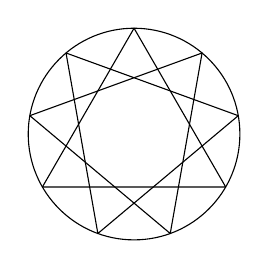
\begin{tikzpicture}[scale=0.56,line cap=round,line join=round]
  \draw (0,0) circle (2.4);
  \foreach \r in {-40,0,40} {
    \draw ({90+\r}:2.4)--({210+\r}:2.4)--({330+\r}:2.4)--cycle;
  }
\end{tikzpicture}\par}

\begin{choices}
  \choice{27}
  \choice{30}
  \choice{25}
  \choice{32}
  \choice{35}
\end{choices}
\end{question}

\begin{question}{7}{5}
数列满足 \(a_1=5\)，且从第1项开始，每后一项都等于前一项的2倍再加1。\(a_{20}+a_{21}\) 除以7的余数是多少？
\begin{choices}
  \choice{3}
  \choice{4}
  \choice{5}
  \choice{6}
\end{choices}
\end{question}

\begin{question}{8}{5}
当哲哲在下午5:00之后不久开始慢跑时，他注意到他的指针式手表的时针和分针形成了一个 \(99^\circ\) 的夹角。当他在下午6:00之前结束慢跑时，他发现两根指针再次形成了一个 \(99^\circ\) 的夹角。请问哲哲慢跑了多少分钟？

% Source figure: assets/original/page-08.png
{\centering
\begin{tikzpicture}[scale=0.98,>=Stealth,line cap=round,line join=round]
  \begin{scope}[xshift=-3.85cm]
    \draw (0,0) circle (2);
    \foreach \a in {0,30,...,330} {
      \draw (\a:1.82)--(\a:2);
    }
    \foreach \n/\a in {12/90,1/60,2/30,3/0,4/-30,5/-60,6/-90,7/-120,8/-150,9/180,10/150,11/120} {
      \node[font=\bfseries\small] at (\a:1.55) {\n};
    }
    \fill (0,0) circle (1.5pt);
    \draw[->,thick] (0,0)--(34.4:1.55);
    \draw[->,thick] (0,0)--(-64.6:1.08);
    \draw[->] (-64.6:0.52) arc[start angle=-64.6,end angle=34.4,radius=0.52];
    \node[font=\small] at (-14:0.82) {\(99^\circ\)};
  \end{scope}
  \begin{scope}[xshift=3.85cm]
    \draw (0,0) circle (2);
    \foreach \a in {0,30,...,330} {
      \draw (\a:1.82)--(\a:2);
    }
    \foreach \n/\a in {12/90,1/60,2/30,3/0,4/-30,5/-60,6/-90,7/-120,8/-150,9/180,10/150,11/120} {
      \node[font=\bfseries\small] at (\a:1.55) {\n};
    }
    \fill (0,0) circle (1.5pt);
    \draw[->,thick] (0,0)--(178.4:1.55);
    \draw[->,thick] (0,0)--(-82.6:1.08);
    \draw[->] (-82.6:0.52) arc[start angle=-82.6,end angle=-181.6,radius=0.52];
    \node[font=\small] at (-133:0.82) {\(99^\circ\)};
  \end{scope}
\end{tikzpicture}\par}

\begin{choices}
  \choice{34}
  \choice{35}
  \choice{36}
  \choice{37}
  \choice{38}
\end{choices}
\end{question}

\begin{question}{9}{5}
正数 \(a,b\) 满足 \(a+b=18\)，且 \(\dfrac{a}{b}+\dfrac{b}{a}=\dfrac{5}{2}\)。\(ab\) 等于多少？
\begin{choices}
  \choice{60}
  \choice{66}
  \choice{72}
  \choice{78}
\end{choices}
\end{question}

\begin{question}{10}{5}
用数字1、2、3、4、5、6中的4个不同数字排成一列，要求前两个数字之和大于后两个数字之和。共有多少种排法？
\begin{choices}
  \choice{144}
  \choice{148}
  \choice{152}
  \choice{156}
\end{choices}
\end{question}

\sectionbanner{多选题}{共4题，每题7分，共28分}

\begin{question}{11}{7}
每套书签12元，每盒彩笔8元。小林两种都买，共花96元。判断下列说法中哪些一定正确。
\begin{multichoices}
  \choice{书签的套数一定是偶数}
  \choice{彩笔的盒数可以是5}
  \choice{两种物品一共可以买10件}
  \choice{书签最多可以买6套}
\end{multichoices}
\end{question}

\begin{question}{12}{7}
设 \(N=2^3\times3^2\times5\)。判断下列说法中哪些一定正确。
\begin{multichoices}
  \choice{\(N\) 有24个正因数}
  \choice{\(N\) 有6个奇正因数}
  \choice{\(N\) 的正因数中，能被15整除的有8个}
  \choice{\(N\) 的正因数中，完全平方数有6个}
\end{multichoices}
\end{question}

\begin{question}{13}{7}
三堆棋子分别有7枚、10枚、13枚。每次操作选择一堆放入2枚棋子，同时从另外两堆各取走1枚棋子。判断下列说法中哪些一定正确。
\begin{multichoices}
  \choice{三堆棋子的总数始终不变}
  \choice{有奇数枚棋子的堆数始终是偶数}
  \choice{可以经过若干次操作后使三堆棋子都为10枚}
  \choice{每一堆棋子数的奇偶性都保持不变}
\end{multichoices}
\end{question}

\begin{question}{14}{7}
正整数 \(a,b\) 满足 \(a+b=18\)。判断下列说法中哪些一定正确。
\begin{multichoices}
  \choice{\(ab\) 的最大值是81}
  \choice{\(a^2+b^2\) 一定是偶数}
  \choice{如果 \(ab\) 能被17整除，那么 \(a,b\) 中有一个数是17}
  \choice{\(ab\) 可以等于70}
\end{multichoices}
\end{question}

\sectionbanner{二、填空题}{共5题，每题6分，共30分}

\begin{question}{15}{6}
从1到12中任取两个不同的数，使它们的和能被3整除。不计顺序，这样的取法有\underline{\hspace{1.35cm}}种。
\end{question}

\begin{question}{16}{6}
在一个 \(3\times6\) 的表格中，有多少对儿单位正方形没有公共点？图中显示了满足条件的其中一对儿。

% Source figure: assets/original/page-16.png
\noindent
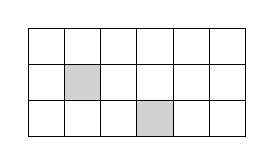
\begin{tikzpicture}[x=0.46cm,y=0.46cm]
  \fill[gray!35] (1,1) rectangle (2,2);
  \fill[gray!35] (3,0) rectangle (4,1);
  \draw[step=1] (0,0) grid (6,3);
\end{tikzpicture}

\end{question}

\begin{question}{17}{6}
黑板上写着1到30这30个整数。每次擦去两个数，再写上这两个数的和。重复操作直到黑板上只剩一个数。最后剩下的数是 \answerline。
\end{question}

\begin{question}{18}{6}
一个正方形被两条线分成了四块。已知其中三块的面积分别是 \(350\text{ m}^2\)、\(163\text{ m}^2\)、\(56\text{ m}^2\)，求最后一块（顶部四边形）的面积是多少平方米？

% Source figure: assets/original/page-18.png
\noindent
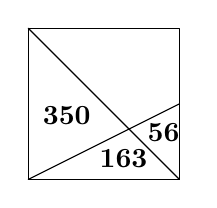
\begin{tikzpicture}[line cap=round,line join=round,scale=0.48]
  \coordinate (P) at (2.86,1.43);
  \draw (0,0) rectangle (4,4);
  \draw (0,4)--(4,0);
  \draw (0,0)--(4,2.00);
  \node[font=\bfseries] at (1.02,1.70) {350};
  \node[font=\bfseries] at (2.52,0.55) {163};
  \node[font=\bfseries] at (3.58,1.25) {56};
\end{tikzpicture}

\end{question}

\enlargethispage{8mm}
\begin{question}{19}{6}
9个互不相同的正整数的平均数为18，其中最小的数是6。这些数中最大数的最小可能值是 \answerline。
\end{question}

\sectionbanner{三、综合题}{共3题，每题14分，共42分}

\begin{question}{20}{14}
标有1到7数字的正六边形灯按右图排列。按下每个灯时，点亮和熄灭的状态会按照以下规则进行切换：

% Source figure: assets/original/page-20.png
{\centering
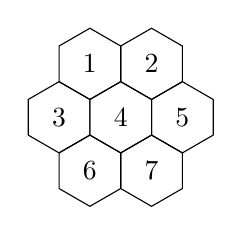
\begin{tikzpicture}[scale=0.78,line cap=round,line join=round]
  \foreach \x/\y/\n in {-0.502/0.87/1,0.502/0.87/2,-1.004/0/3,0/0/4,1.004/0/5,-0.502/-0.87/6,0.502/-0.87/7} {
    \draw ({\x},{\y+0.58})--({\x+0.502},{\y+0.29})--
          ({\x+0.502},{\y-0.29})--({\x},{\y-0.58})--
          ({\x-0.502},{\y-0.29})--({\x-0.502},{\y+0.29})--cycle;
    \node at (\x,\y) {\n};
  }
\end{tikzpicture}\par}

被按下的灯，其点亮/熄灭状态切换。

在与被按下的灯相邻的灯中，只有数字大于被按下的灯，其状态才会切换。

例如，如下方图示，当只有1和7号灯亮着时，按3、2的顺序按下灯，最后1，2，3，5，6，7号灯会处于点亮状态。

% Source figure: assets/original/page-20.png
{\centering
\begin{tikzpicture}[scale=0.50,>=Stealth,line cap=round,line join=round]
  \begin{scope}[xshift=0cm]
    \foreach \x/\y/\n/\lit in {-0.502/0.87/1/1,0.502/0.87/2/0,-1.004/0/3/0,0/0/4/0,1.004/0/5/0,-0.502/-0.87/6/0,0.502/-0.87/7/1} {
      \ifnum\lit=1
        \path[pattern=north east lines,pattern color=gray!75]
          ({\x},{\y+0.58})--({\x+0.502},{\y+0.29})--
          ({\x+0.502},{\y-0.29})--({\x},{\y-0.58})--
          ({\x-0.502},{\y-0.29})--({\x-0.502},{\y+0.29})--cycle;
      \fi
      \draw ({\x},{\y+0.58})--({\x+0.502},{\y+0.29})--
            ({\x+0.502},{\y-0.29})--({\x},{\y-0.58})--
            ({\x-0.502},{\y-0.29})--({\x-0.502},{\y+0.29})--cycle;
      \node at (\x,\y) {\n};
    }
  \end{scope}
  \draw[->] (1.6,0)--node[above] {按下3} (3.0,0);
  \begin{scope}[xshift=4.6cm]
    \foreach \x/\y/\n/\lit in {-0.502/0.87/1/1,0.502/0.87/2/0,-1.004/0/3/1,0/0/4/1,1.004/0/5/0,-0.502/-0.87/6/1,0.502/-0.87/7/1} {
      \ifnum\lit=1
        \path[pattern=north east lines,pattern color=gray!75]
          ({\x},{\y+0.58})--({\x+0.502},{\y+0.29})--
          ({\x+0.502},{\y-0.29})--({\x},{\y-0.58})--
          ({\x-0.502},{\y-0.29})--({\x-0.502},{\y+0.29})--cycle;
      \fi
      \draw ({\x},{\y+0.58})--({\x+0.502},{\y+0.29})--
            ({\x+0.502},{\y-0.29})--({\x},{\y-0.58})--
            ({\x-0.502},{\y-0.29})--({\x-0.502},{\y+0.29})--cycle;
      \node at (\x,\y) {\n};
    }
  \end{scope}
  \draw[->] (6.2,0)--node[above] {按下2} (7.6,0);
  \begin{scope}[xshift=9.2cm]
    \foreach \x/\y/\n/\lit in {-0.502/0.87/1/1,0.502/0.87/2/1,-1.004/0/3/1,0/0/4/0,1.004/0/5/1,-0.502/-0.87/6/1,0.502/-0.87/7/1} {
      \ifnum\lit=1
        \path[pattern=north east lines,pattern color=gray!75]
          ({\x},{\y+0.58})--({\x+0.502},{\y+0.29})--
          ({\x+0.502},{\y-0.29})--({\x},{\y-0.58})--
          ({\x-0.502},{\y-0.29})--({\x-0.502},{\y+0.29})--cycle;
      \fi
      \draw ({\x},{\y+0.58})--({\x+0.502},{\y+0.29})--
            ({\x+0.502},{\y-0.29})--({\x},{\y-0.58})--
            ({\x-0.502},{\y-0.29})--({\x-0.502},{\y+0.29})--cycle;
      \node at (\x,\y) {\n};
    }
  \end{scope}
\end{tikzpicture}\par}

在此规则下，请回答以下问题：

\subquestion{4}{假设所有灯最初都是熄灭的。如果按1、5、6的顺序按下灯，请写出所有点亮的灯的数字之和为多少？}
\answerspace

\subquestion{5}{假设最初只有2号灯亮着。为了让所有灯都熄灭，至少需要按3次灯。请给出一个按3次就能让灯全灭的操作顺序。（将按下的数从小到大排列，直接写三个数字，中间不需要标点或空格）}
\answerspace

\subquestion{5}{假设最初只有1，4，6号灯亮着。为了让所有灯都熄灭，至少需要按5次灯。请给出一个按5次就能让灯全灭的操作顺序。（将按下的数从小到大排列，直接写五个数字，中间不需要标点或空格）}
\answerspace
\end{question}

\begin{question}{21}{14}
依次投掷红色和绿色的2个骰子，将掷出的点数分别记为 \(A,B\)。不过，骰子的点数是从1到6各一个。此时，我们要计算使得 \(A\times B\) 等于某个特定数值的掷出方法有多少种。例如，使得 \(A\times B=8\) 的掷出方法有 \(A=2,B=4\) 和 \(A=4,B=2\)，共2种。

\subquestion{4}{使得 \(A\times B=[\text{学}]\) 的掷出方法总共有4种。请写出所有符合条件的 \([\text{学}]\) 的数值和。}
\answerspace

\subquestion{5}{使得 \(A\times B=[\text{好}]\) 的掷出方法总共有2种。请问符合条件的 \([\text{好}]\) 的数值共有多少个？}
\answerspace

\subquestion{5}{依次投掷红色、绿色、蓝色、黄色的4个骰子，将掷出的点数分别记为 \(A,B,C,D\)。使得 \(A\times B=C\times D\) 的掷出方法总共有多少种？}
\answerspace
\end{question}

\begin{question}{22}{14}
有一座以 \(T\) 点为顶点的五角锥形山。如图所示，五角锥的所有边都是道路，并且在山高的 \(\dfrac13\) 和 \(\dfrac23\) 处也有五边形的道路。在 \(A\) 点和 \(B\) 点之间有一个展望台，在 \(C\) 点和 \(D\) 点之间有一个茶屋。从 \(S\) 点出发，通过某条道路前往 \(T\) 点。但是，不能经过同一个地点或同一条道路，也不能从上往下走。

% Source figure: assets/original/page-26.png
\begin{center}
\begin{tikzpicture}[scale=0.60,line cap=round,line join=round]
  \coordinate (T)  at (2.0,4.3);
  \coordinate (S)  at (5.4,0);
  \coordinate (V2) at (3.3,-1.2);
  \coordinate (V3) at (-0.7,-0.75);
  \coordinate (V4) at (-1.5,1.15);
  \coordinate (V5) at (1.4,1.65);

  \coordinate (A)  at (4.267,1.433);
  \coordinate (A2) at (2.867,0.633);
  \coordinate (A3) at (0.2,0.933);
  \coordinate (C)  at (-0.333,2.2);
  \coordinate (A5) at (1.6,2.533);

  \coordinate (B)  at (3.133,2.867);
  \coordinate (B2) at (2.433,2.467);
  \coordinate (B3) at (1.1,2.617);
  \coordinate (D)  at (0.833,3.25);
  \coordinate (B5) at (1.8,3.417);

  % Base and five rising edges
  \draw (S)--(V2)--(V3)--(V4)--(V5)--cycle;
  \draw (S)--(A)--(B)--(T);
  \draw (V2)--(A2)--(B2)--(T);
  \draw (V3)--(A3)--(B3)--(T);
  \draw (V4)--(C)--(D)--(T);
  \draw[dashed] (V5)--(A5)--(B5)--(T);

  % Roads at one-third height
  \draw (A)--(A2)--(A3)--(C);
  \draw[dashed] (C)--(A5)--(A);

  % Roads at two-thirds height
  \draw (B)--(B2)--(B3)--(D);
  \draw[dashed] (D)--(B5)--(B);

  \foreach \p in {T,S,V2,V3,V4,V5,A,A2,A3,C,A5,B,B2,B3,D,B5} {
    \fill (\p) circle (1.6pt);
  }

  \node[above] at (T) {\(T\)};
  \node[right] at (S) {\(S\)};
  \node[right] at (A) {\(A\)};
  \node[right] at (B) {\(B\)};
  \node[left] at (C) {\(C\)};
  \node[left] at (D) {\(D\)};
  \node[above left=1pt and 2pt of C] {茶屋};
  \node[right=5pt of A] {展望台};
\end{tikzpicture}
\end{center}

\subquestion{4}{如果规定必须经过 \(A,B\) 之间的展望台，从 \(S\) 到 \(A\) 的走法有 \([\text{数}]\) 种，从 \(B\) 到 \(T\) 的走法有 \([\text{学}]\) 种，因此，从 \(S\) 到 \(T\) 并经过展望台的走法有 \([\text{数}]\times[\text{学}]\) 种。\([\text{数}]\times[\text{学}]\) 是多少？}
\answerspace

\subquestion{5}{如果规定必须经过 \(C,D\) 之间的茶屋，从 \(S\) 到 \(C\) 的走法有 \([\text{语}]\) 种，从 \(D\) 到 \(T\) 的走法有 \([\text{文}]\) 种，因此，从 \(S\) 到 \(T\) 并经过茶屋的走法有 \([\text{语}]\times[\text{文}]\) 种。\([\text{语}]\times[\text{文}]\) 是多少？}
\answerspace

\subquestion{5}{从 \(S\) 到 \(T\) 的总走法有几种？}
\answerspace
\end{question}
